\usepackage{lipsum}

\usepackage{graphicx}
\usepackage{float}
\usepackage{booktabs}

\begin{document}

% =======================================================================================
%\cleardoublepage % Forces the first chapter to start on an odd page so it's on the right

% =======================================================================================
%                                   PREAMBLE
% =======================================================================================
\coverpage{\TITLE}{\SUBTITLE}{\AUTHOR}{\DATE}{\SUBJECT}
%----------------------------------------------------------------------------------------
\newpage
\tableofcontents

% =======================================================================================
%                                   PART I
% =======================================================================================
\part{Executive Summary}
%----------------------------------------------------------------------------------------
\newpage
\chapter{Executive Summary} \label{ch:lorem}
In today's data-driven world, managing and processing vast amounts of data efficiently is crucial for organizations across industries. Our innovative data reduction technology addresses this challenge by offering a sustainable and highly efficient solution. By leveraging cutting-edge algorithms, our technology significantly reduces the size of datasets while maintaining data integrity and quality.

{\textbf Key Benefits}

\begin{itemize}
\item Sustainability: Our technology plays a pivotal role in environmental sustainability by reducing the need for extensive data storage infrastructure and minimizing energy consumption during data processing and transmission. This results in a reduced carbon footprint and aligns with global initiatives for sustainable business practices.

\item Efficiency for AI Models: By employing advanced algorithms tailored for AI datasets, our technology enhances the efficiency of model training and inference processes. It accelerates data access and reduces latency, enabling AI models to process information faster and deliver more responsive insights.

\item Efficiency: Through advanced algorithms, our solution enhances operational efficiency. It enables faster data retrieval and processing speeds, thereby improving overall system performance and reducing operational costs associated with data management and processing.

\item Scalability: Designed to scale seamlessly with growing data volumes, our technology caters to the evolving needs of diverse industries such as healthcare, finance, telecommunications, and specially data centers. It ensures that organizations can efficiently manage increasing data loads without compromising on performance or reliability.

\end{itemize}

{\textbf Market Impact}

Our data size reduction technology addresses a critical gap in the market for sustainable data management solutions. By enabling organizations to optimize their data storage and processing capabilities, it positions them to make informed decisions faster and gain a competitive edge in their respective markets. The technology's ability to reduce costs associated with data storage and energy consumption further enhances its attractiveness to businesses seeking operational efficiencies.

Our  technology has a profound impact on the market by addressing fundamental challenges in data management  while fostering sustainable business practices:

\begin{itemize}
\item Competitive Advantage: Organizations adopting our technology gain a competitive edge by optimizing their data management capabilities. They can leverage insights from streamlined data processes to make informed decisions faster, innovate product offerings, and respond swiftly to market demands.
\item Cost Savings: Reduced data storage requirements and lower energy consumption lead to significant cost savings over time. Organizations can reallocate resources towards strategic initiatives such as research and development, customer experience enhancements, or expanding market reach.
\item Compliance and Risk Management: Our technology helps businesses mitigate risks associated with data breaches and non-compliance with data protection regulations. By ensuring data security and integrity, organizations can avoid legal penalties and reputational damage.

\end{itemize}

{\textbf Conclusion}

In conclusion, our data technology represents a transformative advancement in data management practices. By offering sustainable solutions that reduce data footprint while enhancing operational efficiency and scalability, we empower organizations to unlock the full potential of their data assets. Embracing our technology not only supports environmental sustainability but also drives business growth and innovation in an increasingly digital landscape.

For further information on implementation strategies and how our technology can benefit your organization, please contact us. Together, we can embark on a journey towards smarter, more sustainable data management practices.
%----------------------------------------------------------------------------------------
%\newpage
%\chapter{Ipsum}\label{ch:ipsum}
%\section{Proin nec metus venenatis} \label{sec:proin}

Condimentum quam sed, auctor diam. Fusce at bibendum nunc. Vestibulum ut justo
volutpat, placerat turpis at, ultrices lacus. Phasellus blandit fermentum tincidunt.

Quisque eget est ullamcorper massa vestibulum facilisis eget non quam. Pellentesque
eleifend augue vel elit mattis, ut porta risus sodales. Suspendisse vitae odio
facilisis, venenatis leo ut, consequat turpis.

\subsection{Integer magna quam}

In hac habitasse platea dictumst. Pellentesque a hendrerit mauris, ac congue
erat. Maecenas in lorem non velit euismod volutpat. Morbi et arcu quam. Mauris
id scelerisque est. Cras a nunc in justo blandit dictum nec ut tortor.

%\begin{figure}[hb]
%\centering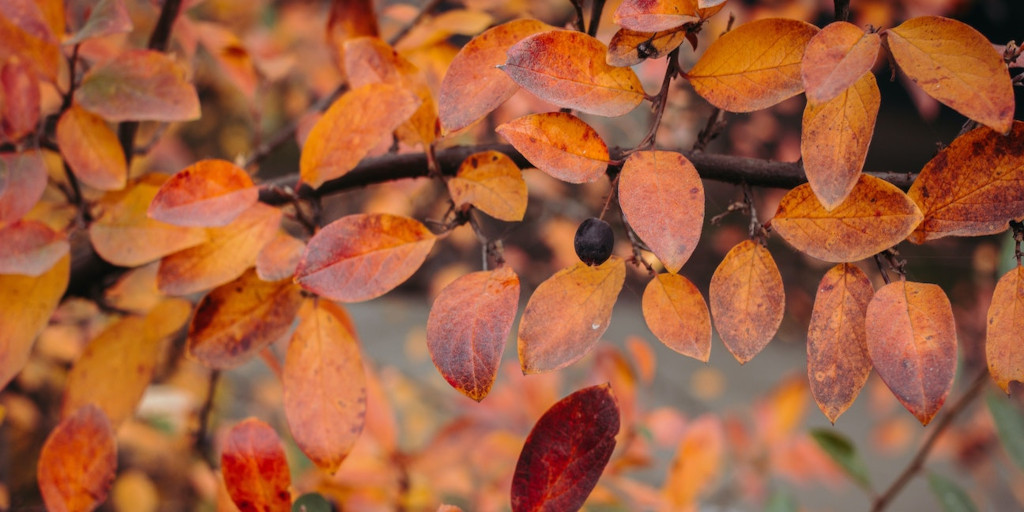
\includegraphics[scale=1]{images/orange2.jpg}
%\caption{Maecenas varius orci vitae eros euismod placerat} %\label{fig:integer}
%\end{figure}

\subsection{Convallis quis elementum feugiat}

Rutrum in ligula. Nulla ut semper ligula, sed lobortis enim. Vivamus nulla eros,
faucibus ac convallis in, ornare at elit. Aliquam erat odio, finibus at purus ut,
porta ullamcorper odio. Vivamus ac augue tincidunt, semper magna volutpat,
condimentum sem. Praesent eget neque vitae odio volutpat vulputate.


% =======================================================================================
%                                   PART II
% =======================================================================================
% =======================================================================================


\part{Market}
%----------------------------------------------------------------------------------------
\newpage
\chapter{Market} \label{ch:hendrerit}
\input{sections/part2/sustainability}
\newpage
%\section{Sed ultrices} \label{sec:sed-ultrices}

\subsection{Donec pellentesque}

Tempus ipsum, vitae condimentum nisi efficitur id. In velit mauris, auctor eget
sapien nec, viverra mattis neque. Nunc vel commodo nunc, eget cursus ex.

\begin{enumerate}
\item{Nunc maximus consequat tristique.}
\item{Praesent luctus ex aliquam rhoncus consectetur.}
\item{Suspendisse mattis velit ante, vitae mollis est pharetra a.}
\item{Duis tincidunt, urna id auctor imperdiet, odio dui ullamcorper nisi.}
\item{Integer tincidunt enim vitae nulla iaculis, in varius metus blandit.}
\item{Nunc quam arcu, fermentum non dapibus condimentum, condimentum eget nunc.}
\end{enumerate}

\subsection{Euismod sodales}

Removed

\subsection{Pellentesque a nulla}

Removed
%\newpage
%\section{Sed ultrices} \label{sec:sed-ultrices}

\subsection{Donec pellentesque}

Tempus ipsum, vitae condimentum nisi efficitur id. In velit mauris, auctor eget
sapien nec, viverra mattis neque. Nunc vel commodo nunc, eget cursus ex.

\begin{enumerate}
\item{Nunc maximus consequat tristique.}
\item{Praesent luctus ex aliquam rhoncus consectetur.}
\item{Suspendisse mattis velit ante, vitae mollis est pharetra a.}
\item{Duis tincidunt, urna id auctor imperdiet, odio dui ullamcorper nisi.}
\item{Integer tincidunt enim vitae nulla iaculis, in varius metus blandit.}
\item{Nunc quam arcu, fermentum non dapibus condimentum, condimentum eget nunc.}
\end{enumerate}

\subsection{Euismod sodales}

Removed

\subsection{Pellentesque a nulla}

Removed

% =======================================================================================
\part{Technology}
%----------------------------------------------------------------------------------------
\newpage
\chapter{Data Reduction} \label{ch:hendrerit}
\section{The goal}

The aim of data reduction is to simplify a dataset while preserving its key information. This can typically be accomplished by either reducing the number of features or the number of samples. Our approach will concentrate on the more challenging task of reducing the sample size.

\section{Need for data size reduction}

With data being collected at an unprecedented pace, data reduction plays a critical role in boosting training efficiency. By reducing the number of samples, we create a simpler yet representative dataset, which can alleviate memory and computation constraints. This not only enhances sustainability by lowering energy consumption but also contributes to significant energy savings.

\section{Regular methods for reducing sample size}

Sample reduction is typically achieved through instance selection, which involves choosing a representative subset of data samples that retain the original dataset's properties. Existing methods can be categorized into wrapper and filter methods. Filter methods select instances based on scoring functions, such as selecting border instances that often shape the decision boundary. Wrapper methods, on the other hand, select instances based on model performance, considering their interaction with the model. Additionally, instance selection techniques can address data imbalance issues by undersampling the majority class, such as with random undersampling. Recent advancements have incorporated reinforcement learning to optimize undersampling strategies. However, these regular methods neither achieve the data size reduction nor the accuracy level that our data size reduction approach can deliver.

\section{Challenges}

The challenges of data reduction are twofold. First, selecting the most representative data or projecting data into a low-dimensional space with minimal information loss is complex. While learning-based methods can partially address these challenges, they often require substantial computational resources, particularly with very large datasets. Consequently, achieving both high accuracy and efficiency is difficult. Second, data reduction can potentially amplify data bias, raising fairness concerns.
\chapter{Validation Tests} \label{ch:hendrerit}
\section{Introduction}

In the realm of data science and machine learning, the efficiency and effectiveness of data processing are often contingent upon the size and manageability of the datasets in use. The burgeoning volume of data necessitates innovative methods for reducing dataset size without compromising the integrity and utility of the data. This chapter focuses on validation tests for a revolutionary data size reduction method, applied to four well-known datasets: the Iris dataset, the Wine dataset, the Breast Cancer dataset, and the MNIST dataset.

\section{Tests done}
\subsection{Iris Dataset}

The Iris dataset, introduced by Ronald A. Fisher in 1936, is a staple in the field of machine learning and statistics. It consists of 150 instances of iris flowers, each described by four features: sepal length, sepal width, petal length, and petal width. These features are used to classify the flowers into three species: Iris-setosa, Iris-versicolor, and Iris-virginica. The simplicity and clarity of the Iris dataset make it an ideal candidate for demonstrating basic principles of data size reduction.

\begin{figure}[h]
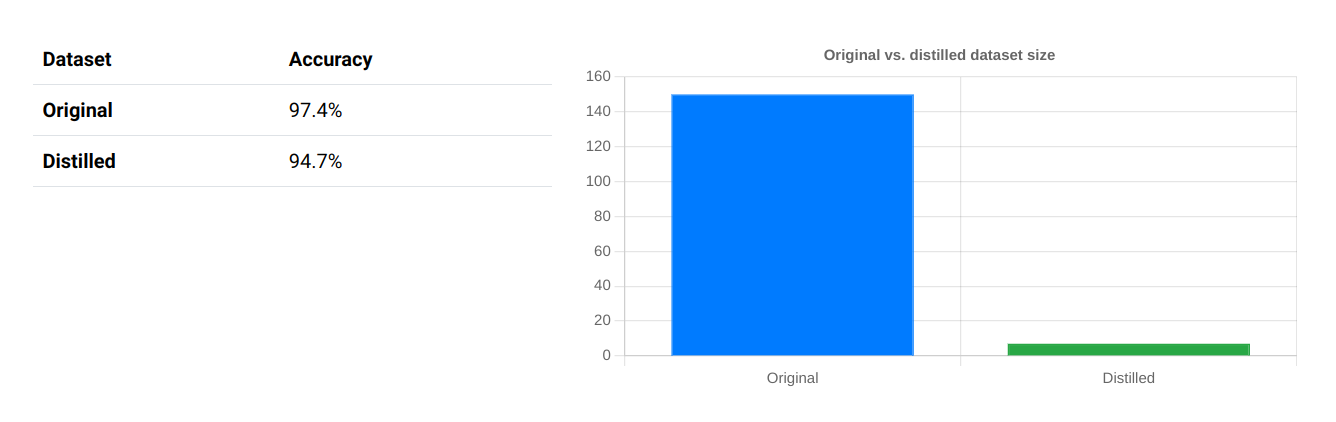
\includegraphics[width=0.9\textwidth]{images/Iris_validation_test.png}
\centering
\caption{}
\end{figure}

\subsection{Wine Dataset}

The Wine dataset is derived from the results of a chemical analysis of wines grown in the same region in Italy but derived from three different cultivars. It contains 178 instances with 13 attributes including alcohol content, malic acid, ash, and others. This dataset is often used for classification problems and serves as an excellent test bed for validating data reduction techniques due to its moderate size and complexity.

\begin{figure}[h]
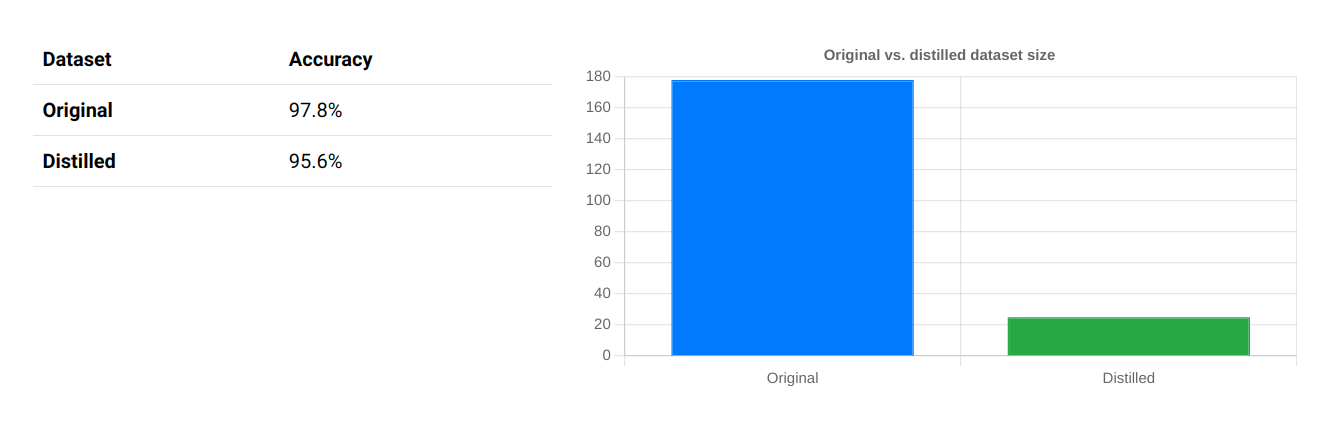
\includegraphics[width=0.9\textwidth]{images/Wine_validation_test.png}
\centering
\caption{}
\end{figure}

\subsection{Breast Cancer Dataset}

The Breast Cancer Wisconsin dataset, created by Dr. William H. Wolberg, is used for binary classification tasks in predicting the malignancy of breast cancer samples. It comprises 569 instances, each with 30 numeric features representing characteristics of cell nuclei present in a digitized image of a fine needle aspirate of a breast mass. This dataset is critically important for medical research and diagnostics, making the preservation of data quality essential during size reduction.

\begin{figure}[h]
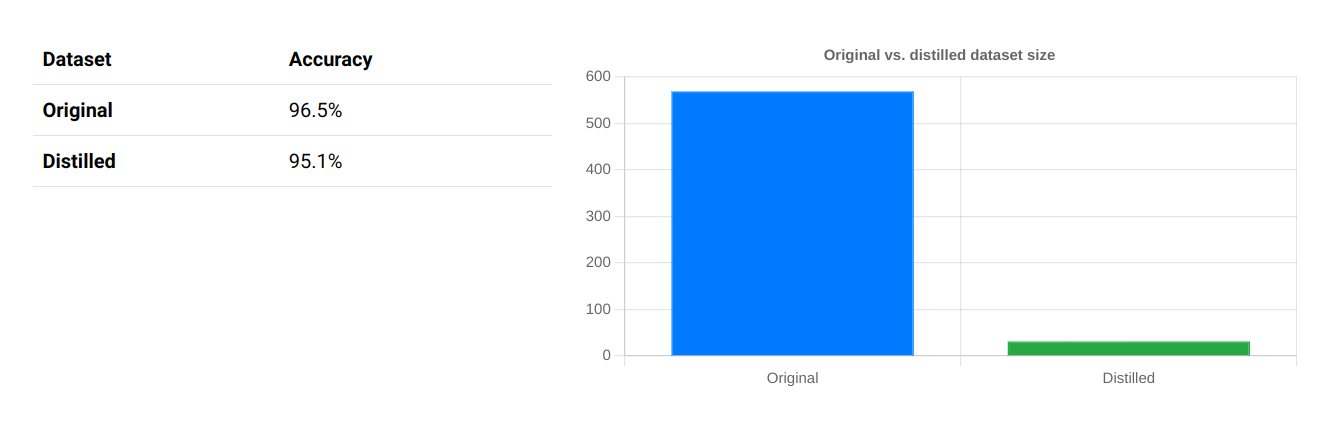
\includegraphics[width=0.9\textwidth]{images/Breast_validation_test.png}
\centering
\caption{}
\end{figure}

\subsection{MNIST Dataset}

The MNIST dataset is a large collection of handwritten digits, commonly used for training various image processing systems. It includes 60,000 training examples and 10,000 testing examples, each represented by a 28x28 grayscale image of a digit (0-9). The high dimensionality and substantial size of the MNIST dataset present significant challenges for data size reduction, thus providing a rigorous test for our proposed method.

\begin{figure}[h]
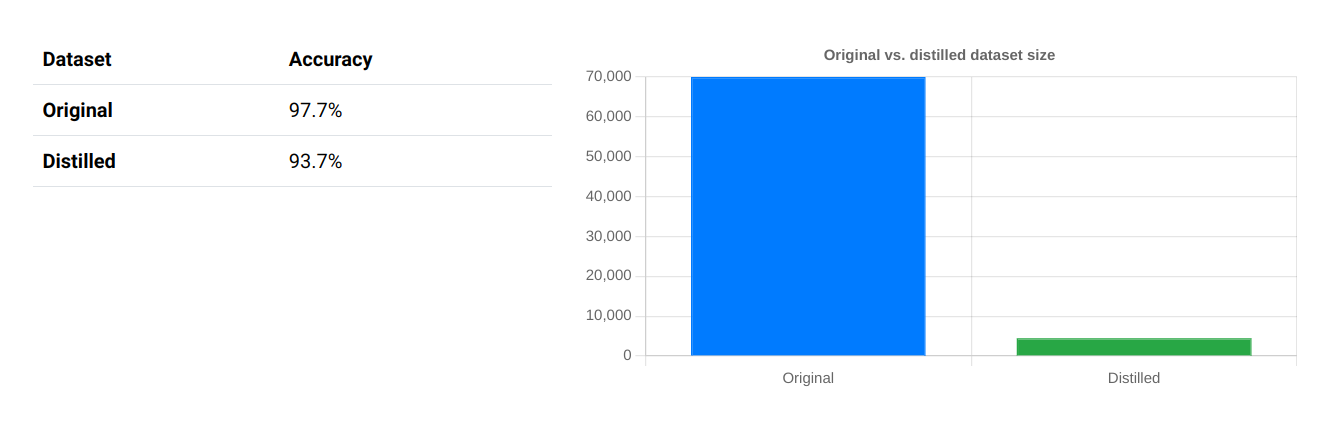
\includegraphics[width=0.9\textwidth]{images/MNIST_validation_test.png}
\centering
\caption{}
\end{figure}

% =======================================================================================
\part{Business model}
%----------------------------------------------------------------------------------------
\newpage
\chapter{Hendrerit sapien} \label{ch:hendrerit}
\section{Sed ultrices} \label{sec:sed-ultrices}

\subsection{Donec pellentesque}

Tempus ipsum, vitae condimentum nisi efficitur id. In velit mauris, auctor eget
sapien nec, viverra mattis neque. Nunc vel commodo nunc, eget cursus ex.

\begin{enumerate}
\item{Nunc maximus consequat tristique.}
\item{Praesent luctus ex aliquam rhoncus consectetur.}
\item{Suspendisse mattis velit ante, vitae mollis est pharetra a.}
\item{Duis tincidunt, urna id auctor imperdiet, odio dui ullamcorper nisi.}
\item{Integer tincidunt enim vitae nulla iaculis, in varius metus blandit.}
\item{Nunc quam arcu, fermentum non dapibus condimentum, condimentum eget nunc.}
\end{enumerate}

\subsection{Euismod sodales}

Removed

\subsection{Pellentesque a nulla}

Removed
\newpage
\section{Sed ultrices} \label{sec:sed-ultrices}

\subsection{Donec pellentesque}

Tempus ipsum, vitae condimentum nisi efficitur id. In velit mauris, auctor eget
sapien nec, viverra mattis neque. Nunc vel commodo nunc, eget cursus ex.

\begin{enumerate}
\item{Nunc maximus consequat tristique.}
\item{Praesent luctus ex aliquam rhoncus consectetur.}
\item{Suspendisse mattis velit ante, vitae mollis est pharetra a.}
\item{Duis tincidunt, urna id auctor imperdiet, odio dui ullamcorper nisi.}
\item{Integer tincidunt enim vitae nulla iaculis, in varius metus blandit.}
\item{Nunc quam arcu, fermentum non dapibus condimentum, condimentum eget nunc.}
\end{enumerate}

\subsection{Euismod sodales}

Removed

\subsection{Pellentesque a nulla}

Removed

% =======================================================================================

\part{Team}
%----------------------------------------------------------------------------------------
\newpage
\chapter{Technology creators} \label{ch:hendrerit}
\section{Members} \label{sec:team}

\subsection{Ivan Romero, PhD}

\begin{figure*}[!ht]
  \centering
  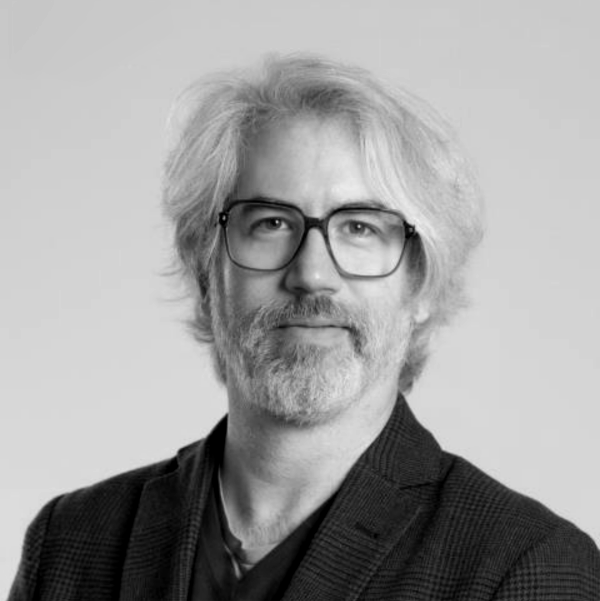
\includegraphics[width=.25\textwidth]{../../img/team/romero.png}
  \caption{}
\end{figure*}

{\small 
Tempus ipsum, vitae condimentum nisi efficitur id. In velit mauris, auctor eget
sapien nec, viverra mattis neque. Nunc vel commodo nunc, eget cursus ex.
}

Contact: \faEnvelope\ \href{mailto:ivanromeroruiz@gmail.com}{ivanromeroruiz@gmail.com}

\subsection{Jose L. Salmeron, PhD}

\begin{figure*}[!ht]
  \centering
  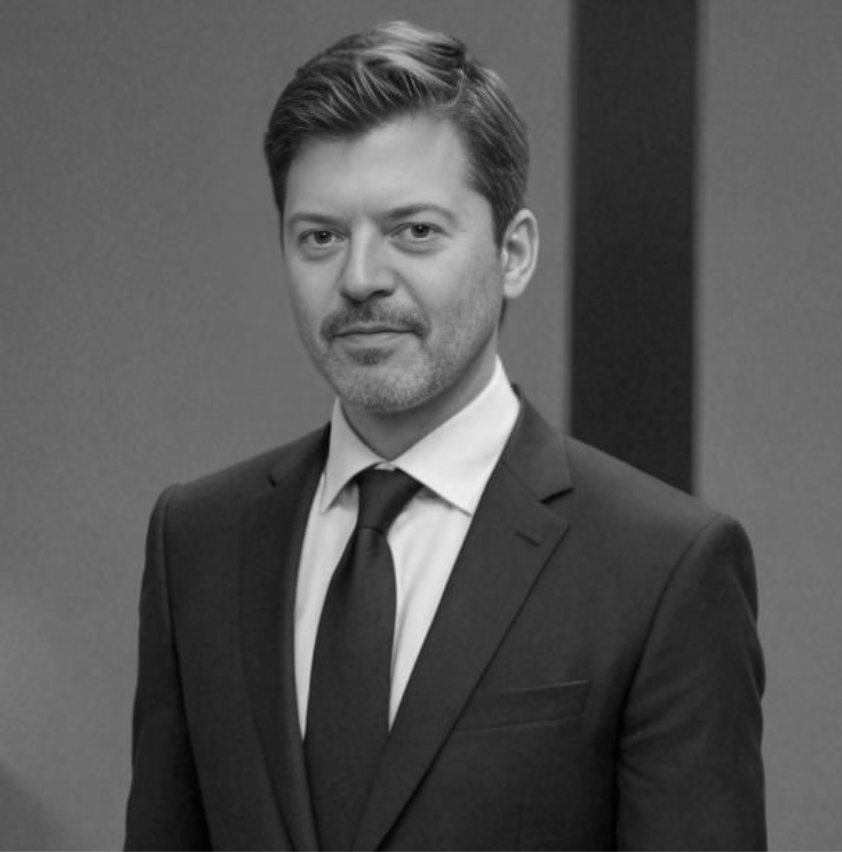
\includegraphics[width=.25\textwidth]{../../img/team/salmeron.png}
  \caption{}
\end{figure*}

{\small 
Prof. Jose L. Salmeron, Ph.D., Eng., ACM Senior Lifetime member has served as Principal AI \& Quantum Scientist at the Hybrid Intelligence division of Capgemini and holds the position of (Catedratico) Professor of Computer Science and Artificial Intelligence at CUNEF University. He has almost 30 years of experience in technology and research, including positions at several universities, consulting in the AI/IT industry, and a wide range of projects with private and public organizations such as Intel, Cisco, Vodafone, Gilead, Microsoft, Airbus, BBVA, and others. He has also been awarded ACM Senior Membership. Prof. Salmeron has consistently been featured in Stanford list of the world’s top 2\% scientists since the initial version. He has authored or co-authored over 200 scientific articles, conference papers, and book chapters indexed in ISI Web of Science. Furthermore, his work has garnered over 5,900 citations from researchers in 20 different countries, resulting in an h-index of 37 on Google Scholar. His primary field of expertise encompass Distributed Artificial Intelligence, eXplainable Artificial Intelligence, Reservoir Computing, Quantum Computing, Causal Machine Learning, and Federated Learning.}

Contact: \faEnvelope\ \href{mailto:joseluis.salmeron@gmail.com}{joseluis.salmeron@gmail.com}
\newpage
%\input{sections/part5/accumsan}

% =======================================================================================

\part{Funding}
%----------------------------------------------------------------------------------------
\newpage
\chapter{Funds requirements and applications} \label{ch:hendrerit}
%\section{Revenue}
The revenue table forecasts profits through 2026. The AI (TWh) field shows the estimated energy demand for AI processes in data centers worldwide, based on predictions from Schneider Electric. The Electricity price (\$) field predicts the average electricity price in the United States. 

The AI cost (B\$) field predicts the global cost of energy demand for AI processes in data centers. The AI energy saved (TWh) field estimates the energy savings from our solution. The Saved cost (B\$) field represents the predicted cost savings due to our solution, and the CO2 saved (Mt) field shows the megatons of $CO_2$ emissions that will be prevented with our solution. SAM (\%) indicates the percentage of market share defining the serviceable addressable market, while SAM (B\$) represents the money saved in the SAM. SOM (M\$) predicts the serviceable obtainable market, which is the estimated profit until 2026 (comission 10\%). Cum. SOM (M\$) is the cumulative predicted profit expected until 2026. Following the upward trend in average electricity prices and the growing demand in data centers, it is estimated that by 2030, SOM benefits will reach at least 606 million dollars.

\begin{table}[!h]
\footnotesize
\begin{tabular}{ccccccccccccc}
\toprule
 & AI & Electricity & AI cost & AI energy  & Saved cost & CO\textsubscript{2}  & SAM & SAM  & SOM  & Cum. \\
Year & (TWh) & price (\$) & (B\$) & saved (TWh) &  (B\$) & saved (Mt) & (\%) &   (M\$) & (M\$) & SOM (M\$) \\
\midrule
2023 & ;40   & 0.170   & 7   & 34  & 6   & 7   & 0.000     & 0     & 0    & 0 \\
2024 & 54  & 0.175  & 9   & 46  & 8   & 10  & 0.000     & 0      & 0    & 0 \\
2025 & 72 & 0.180   & 13  & 62  & 11  & 13  & 0.001 & 11     & 1.1  & 1 \\
2026 & 92 & 0.185  & 17  & 79  & 15  & 16  & 0.007 & 105   & 10.5 & 12 \\
2027 & 115 & 0.190  & 22  & 99  & 19  & 20  & 0.015 & 285   & 28.5 & 40 \\
\bottomrule
\end{tabular}
\caption{Energy demand prevision and costs}
\end{table}

Given the increasing power demand in data centers and the anticipated scarcity of energy in the midterm future, our data size reduction solution should be considered a standard protocol. The adoption of our solution in the algorithmic AI processes of data centers leads to significant energy savings, which translates to substantial cost reductions and a decrease in CO2 emissions. 

As energy demands continue to rise, the necessity for efficient energy solutions becomes more critical. Our solution offers a sustainable path forward, ensuring that data centers can meet the growing needs while minimizing their environmental impact and operational costs. The projected savings and reduced carbon footprint underscore the vital role our solution will play in the future of data center operations. Adopting our data size reduction as a standard protocol is essential for maintaining energy efficiency and sustainability in the face of increasing energy constraints.

\newpage
\section{Sed ultrices} \label{sec:sed-ultrices}

\subsection{Donec pellentesque}

Tempus ipsum, vitae condimentum nisi efficitur id. In velit mauris, auctor eget
sapien nec, viverra mattis neque. Nunc vel commodo nunc, eget cursus ex.

\begin{enumerate}
\item{Nunc maximus consequat tristique.}
\item{Praesent luctus ex aliquam rhoncus consectetur.}
\item{Suspendisse mattis velit ante, vitae mollis est pharetra a.}
\item{Duis tincidunt, urna id auctor imperdiet, odio dui ullamcorper nisi.}
\item{Integer tincidunt enim vitae nulla iaculis, in varius metus blandit.}
\item{Nunc quam arcu, fermentum non dapibus condimentum, condimentum eget nunc.}
\end{enumerate}

\subsection{Euismod sodales}

Removed

\subsection{Pellentesque a nulla}

Removed

% =======================================================================================

%                                   APPENDICES
% =======================================================================================
\part{Appendices}
%----------------------------------------------------------------------------------------
\newpage
\chapter{Vestibulum commodo} \label{ch:commodo}
\section*{Integer semper dictum tellus}

Neque eu cursus faucibus, ipsum magna tincidunt dui, vel scelerisque urna nibh ut nisl:

\begin{description}[labelwidth=\widthof{\bfseries morbi convallis},align=left]
\item[Duis]{sit amet mattis magna.}
\item[Curabitur]{sit amet fermentum mi.}
\item[Morbi convallis]{purus eu fermentum accumsan, mauris felis consequat ipsum.}
\item[Ut]{sollicitudin sit amet tellus et mollis.}
\end{description}

\section*{A porttitor orci faucibus sit amet}

Vivamus et sapien vitae lacus ornare suscipit vitae id mauris:

\begin{description}[labelwidth=\widthof{\bfseries suspendisse},align=left]
\item[Vivamus]{in dui arcu.}
\item[Morbi]{vitae dolor libero.}
\item[Tellus]{est, pellentesque at ultrices non, consectetur sit amet augue.}
\item[Suspendisse]{elementum mollis nisl at aliquam.}
\end{description}

%----------------------------------------------------------------------------------------
\newpage
\chapter{Etiam facilisis} \label{ch:etiam}
\section{Ipsum primis}

In faucibus orci luctus et ultrices posuere cubilia curae; Aliquam nunc ipsum,
sollicitudin ut tempus consectetur, fermentum at lectus.

Nullam molestie viverra \ref{sec:vestibulum} augue sit amet gravida.

\newenvironment{nomenclature}[1]
{
\begin{table}[hbt]
\caption{#1}
\begin{center}
\begin{tabular}{|l|l|l|}
\hline
\textbf{Symbol} & \textbf{Unit} & \textbf{Description}\\
\hline
}
{
\\\hline
\end{tabular}
\end{center}
\end{table}
}

\subsection{Mauris pellentesque}

\begin{nomenclature}{Massa sagittis malesuada}
$g$     & $m/s^{2}$ & nisi in mollis gravida
\end{nomenclature}

\subsection{Nulla massa}

\begin{nomenclature}{Quis imperdiet}
$Q_{p}$         & $t/h$             & consectetur tortor
\end{nomenclature}

\begin{nomenclature}{Magna lectus}
$\tau_{a}$    	& $^{\circ}C$       & integer mollis bibendum gravida\\
$f_{s}$     	& $/jour$           & vestibulum porta urna at ex dignissim tincidunt
\end{nomenclature}

\subsection{Nam vitae}

\begin{nomenclature}{Nibh a lacus tincidunt efficitur}
$X_n$   & $m$               & venenatis nisi\\
$Y_n$   & $m$               & integer malesuada eu ligula nec pharetra\\
$Z_n$   & $m$               & fusce non elit lectus
\end{nomenclature}

%----------------------------------------------------------------------------------------
\newpage
\listoffigures
\listoftables
%----------------------------------------------------------------------------------------
\newpage
\printbibliography[title = {Aliquam}]

\end{document}
